\section{判雷技巧}
本节使用的例子除竞速实战也很常用的定式以外,不会出现在Puzzle中,不用担心剧透。

\subsection{数数}
数数是最基础的判雷规则。如果数字$n$周围已经有了$n$个雷,则剩余格全部安全;如果数字$n$周围只有$n$格不是安全格,则这$n$格都是雷。

\subsection{减法}
扫雷中每个数字实际上代表它周围的区域。两个区域相交时,我们称相交部分为公共格,不相交部分分别是两个区域的独立格。例如下图中,1和2区域相交,A为公共格,C为1侧独立格,D为2侧独立格。1周围比2周围少1雷,所以排除掉公共部分A,可以知道C比D少1雷。这种推理方式叫做减法。
\begin{center}
    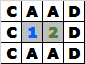
\includegraphics{trick/减法1.png}
\end{center}

另一种思路是,A是1的一部分,所以A中至多1雷;又因为A是2的一部分,所以2周围排除掉A后至少1雷,即D至少一雷,这种思路和之前的思路大同小异,也叫做减法。

我们以竞速实战常用的定式为例介绍减法的用法。

\vspace{5mm}
\begin{center}
    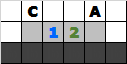
\includegraphics{trick/减法2.png}
\end{center}
上图为12定式,结论是A为雷,C安全。我们分别用两种思路来推导这个结论。
\begin{itemize}
    \item 思路1:A是2侧独立格,C是1侧独立格,$2-1=1$,所以A比C多1雷,所以A为雷,C安全。
    \item 思路2.1:考虑1可以知道21公共的两格至多有1雷,再考虑2,知剩下的一格A为雷,反推知21公共两格有1雷,所以1剩下的一格C安全。
    \item 思路2.2:考虑2可以知道21公共的两格至少有1雷,再考虑1,知剩下的一格C安全,反推知21公共两格有1雷,所以2剩下的一格A为雷。
\end{itemize}
思路2.1和思路2.2实际上一个思路的不同方向,所以我们用减法的时候不用在乎从哪边推起,随便选一边即可。

\vspace{5mm}
\begin{center}
    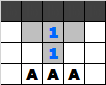
\includegraphics{trick/减法3.png}
\end{center}
上图为挖坑定式,结论是A安全。
\begin{itemize}
    \item 思路1:A是下面1侧独立格,上面1无独立格,$1-1=0$,所以A中无雷。
    \item 思路2:由上面1知两个1公共的两格有1雷,再考虑下面1,知剩下三格均不为雷。
\end{itemize}

思路1和思路2作用略有不同,具体体现在应对连续减法时。

\subsection{连续减法}
我们讲到,减法可以用来推理两个区域之间雷数的关系(思路1),也可以用来推理一个区域中至少或至多有多少雷(思路2)。经过一次减法,得到区域信息,再用这个区域信息去和下一个区域做减法,即叫做连续减法。我们还是通过例子介绍连续减法的用法。

\vspace{5mm}
\begin{center}
    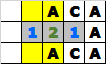
\includegraphics{trick/减法4.png}
\end{center}
上图是121定式。由左边1知黄色区域至多1雷,再考虑2,知C区域至少1雷,再考虑右边1,知A区域全不为雷;反推知C区域有1雷,黄色区域有1雷,左边1的独立格全不为雷。

上述推理过程实际上用了两步减法,第一步是左边12减法得到C至少1雷,第二步是用C和右边1减法得到A全不为雷。为了强调连续减法的方向可以自由选取,我们展示一下如何反向推导。

由右边的1,C区域至多1雷,再考虑2,知黄色区域至少1雷,再考虑左边1,知1侧独立格均不是雷,反推知黄色区域有1雷,C区域有1雷,A区域全不为雷。

\vspace{5mm}
\begin{center}
    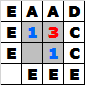
\includegraphics{trick/减法5.png}
\end{center}
上图是角131定式。由左边1知A至多1雷,由下边1知C至多1雷,再考虑3,知D为雷,反推知AC各1雷,E安全。这个例子说明连续减法不一定要从一边单向减到另一边,也可以分头开始。我们展示一下如何把这个分头开始的思路转换成前文的单向连续减法,以说明分头减法也可以看作连续减法。

由左边的1,A区域至多1雷,再考虑3,知CD至少2雷,从而C至少1雷,再考虑下边的1,知下方E安全,反推知C有1雷,D为雷,A有1雷,左侧E安全。

\vspace{5mm}
\begin{center}
    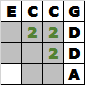
\includegraphics{trick/减法6.png}
\end{center}
上图是角222定式。由左边2知C至少有1雷,由下边2知D至少有1雷,再考虑右上角2知CD各1雷,G安全,反推得AE均为雷。

只要形状允许,连续减法可以不停地连下去。Puzzle212关用到了长达6个数字得连续减法。

\subsection{不等式}
在前文出现的例子中,无论是减法还是连续减法,最终都推出了一些格子一定是雷或一定不是雷的结论。其他一些时候,减法不一定能推出确定的结论,但是由减法得到的区域或格子之间的关系可以帮助我们进一步推导。不等式就是一种利用非确定结论的思路。下面我们(不完全地)列举一些用不等式解题时经常利用的结论,其中大写字母表示区域,小写字母表示单格。

\begin{itemize}
    \item $0\le a\le 1$;$A\ge 0$。
    \item 若$A\ge B$ 且$B\ge C$,则$A\ge C$。
    \item 若$A\ge B$ 且$B\ge A$,则$A=B$。
    \item 若$a+b\le 1$且$a\ge b$,则$b=0$;若$a+b\ge 1$且$a\ge b$,则$a=1$。
    \item 若$A=B+C$,则$A\ge B$且$A\ge C$。
    \item 若$A+B\ge C+D$且$B\le C$,则$A\ge D$。
    \begin{itemize}
        \item 若$A+a=B+1$,则$A\ge B$。
        \item 若$A+a+b=B+2$,则$A\ge B$。
        \item $\dots$
    \end{itemize}
	\item $a=b$当且仅当$a+b=0$或$2$。
\end{itemize}

这些结论从数学角度来说都很显然,所以我们的重点是如何从实战中发现和利用这些结论。请看下面的例子。

\vspace{5mm}
\begin{center}
    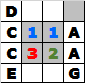
\includegraphics{trick/不等式1.png}
\end{center}
11做减法得到$A=C+D$,$A$区域雷数等于$CD$两块雷数之和,那么自然大于等于其中任何一块,即$A\ge C$且$A\ge D$。

23做减法得到$C+E=A+G+1$,重复前面的技巧,把$G$去掉得到$C+E\ge A+1$。注意到$E$只有一格,所以$E\le 1$,从而$C\ge A$。

回顾我们在第一段得到$A\ge C$,在第二段得到$C\ge A$,从而$A=C$。回顾第一段最开始的$A=C+D$,得$D=0$;回顾第二段最开始的$C+E=A+G+1$,得$E=G+1$,因为$EG$都只有一格,所以$E=1$,$G=0$。

总结一下这个推理过程。在第一段中我们用到了“若$A=B+C$,则$A\ge B$且$A\ge C$”。在第二段中我们用到了“若$A+B\ge C+D$且$B\le C$,则$A\ge D$”的推论“若$A+a=B+1$,则$A\ge B$”。在结尾段我们用到了“若$A\ge B$ 且$B\ge A$,则$A=B$”。这三个命题都是我们刚刚列举过的。下个例子中我们就会省略一些说明,如果读者发现理解有困难,可以回到这个例子复习一下不等式是如何生成的。

\vspace{5mm}
\begin{center}
    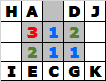
\includegraphics{trick/不等式2.png}
\end{center}
左侧32减法得$A\ge C$(为什么?),右侧21减法得$D\ge C$(为什么?),又因为上中1,$A+D=1$,所以$C=0$(为什么?)。

再次用左侧32减法得$A\ge E$,右侧21减法得$D\ge G$,中列11减法得$A+D=E+G$,所以$A=E$且$D=G$(为什么?)。

再次用左侧32减法得$H=1$,$I=0$;右侧21减法得$J=1$,$K=0$。

\vspace{5mm}比较一下这两个例子。用不等式解局得大致过程都是生成不等式、联系不等式、得到等式、收尾。第一个例子中前两段生成循环的不等式$A\ge C$和$C\ge A$,第三段联系这两个不等式得到等式$A=C$,再重复利用减法得到结论。第二个例子中,第一段就经过了生成不等式、联系不等式、得到等式的过程,但是和第一个例子的区别是,这里生成的不等式是不循环的$A\ge C$和$D\ge C$,所以联系不等式的方式也发生了改变:通过$A+D=1$。第一段得到等式之后也没有简单收尾,而是在第二段重启了整个过程,并且又用了一个新的联系不等式的方法。第三段才是最终的收尾。

不等式的使用是非常灵活的,实战遇到的情况也非常复杂,不可简单概括。掌握了不等式解局之后,扫雷既不是循环套用公式的休闲游戏,也不是暴力穷举的算力游戏,而是充满战术和策略的益智游戏。

不等式在Puzzle中应用非常频繁,在Game中常用来解\nameref{cycle}。我们在最后放一些比较冷门的不等式用法,给读者在\nameref{puzzle}较难关卡遇到困扰时做参考。

\begin{itemize}
	\item $a=b$等价于$a+b=0$或$2$。
	\begin{itemize}
		\item 若$a=b$且$a+b=c+d$,则$a=b=c=d$。
	\end{itemize}
	\item 若$\lambda A\ge B$且$B\le 1$,则$A\ge B$。其中$\lambda$是任何正数。
	\begin{itemize}
		\item 若$A+B\ge C$,$C\le 1$且$A\ge B$,则$A\ge C$。
	\end{itemize}
	\item 若$\lambda A+\mu\ge (\lambda+\mu)B$且$B\le 1$,则$A\ge B$。其中$\lambda$是任何正数,$\mu$是任何实数。
\end{itemize}

\subsection{数雷}
有时我们知道总雷数,相当于知道了整个区域中的雷数。自然地,这个区域也可以和其他区域做减法。因为这个区域最大,所以第一步减法的结果一定是排除掉了一些格子,得到剩下格子的雷数。后续可以进一步排除,也可以当作普通区域做减法等操作。

当剩余雷数为1时,数雷的结论很显然,那就是这个雷必须由所有周围雷数未满的数字共用。反过来,如果剩下的格子只有一个不是雷,那这个安全格也必须由所有周围雷数未满的数字共用。下面举两个实战极其常见的例子。

\vspace{5mm}
\begin{center}
    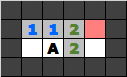
\includegraphics{trick/数雷1.png}
\end{center}
如果剩余1雷,则A为雷。如果剩余2雷,则A不为雷。

\vspace{5mm}
\begin{center}
    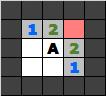
\includegraphics{trick/数雷2.png}
\end{center}
如果剩余1雷,则A为雷。如果剩余3雷,则A不为雷。